\newpage
\begin{center}
    \textbf{\LARGE CHAPTER - 7}
\end{center}
\section{OBSERVATIONS}

\subsection{Time Domain - Gann Chart}
\begin{figure}[H]
	\centering
	 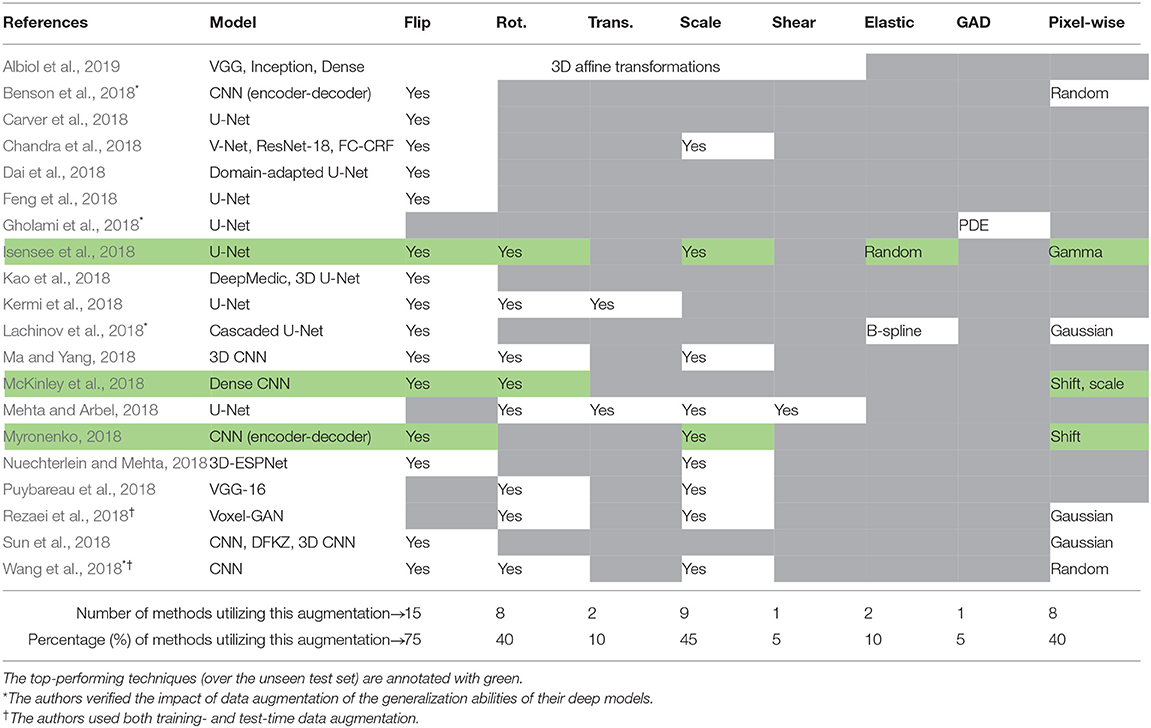
\includegraphics[width=15cm]{ezyzip/img/timegummimage.jpg}
	
	\label{fig:polarization}
\end{figure}	

\subsection{Results and Comparitive Study}
 Several studies have been conducted to explore the effectiveness of Convolutional Neural Networks (CNNs) and transfer learning, particularly using the VGG16 architecture, in the context of brain tumor detection. These studies aim to improve the accuracy and efficiency of brain tumor diagnosis, a critical task in the field of medical imaging.

The VGG16 model, a pre-trained CNN, has been widely adopted in these studies due to its remarkable performance in image classification tasks. Transfer learning with VGG16 involves fine-tuning the network on a new dataset of brain images, thereby leveraging the features learned from a large dataset like ImageNet.

Results from these comparative studies consistently demonstrate the superiority of transfer learning using VGG16 over training CNNs from scratch. This approach exhibits higher accuracy, faster convergence, and the ability to handle limited medical imaging data effectively. Researchers have found that the VGG16-based models can effectively distinguish between tumor and non-tumor regions in brain scans, aiding radiologists in their diagnoses.

Furthermore, transfer learning with VGG16 enables the extraction of meaningful features from brain images, capturing subtle patterns and textures that might be indicative of tumors. This assists in early detection and accurate localization of brain tumors, contributing to better patient outcomes and treatment planning.

In summary, the application of Convolutional Neural Networks, specifically the VGG16 architecture with transfer learning, has proven to be a valuable tool in brain tumor detection. Its ability to harness pre-learned features and adapt to medical imaging datasets has led to improved accuracy and efficiency in diagnosing brain tumors, ultimately benefiting both medical professionals and patients.








